\documentclass[tikz,border=1pt]{standalone}
\usepackage[T1]{fontenc}
\usepackage[utf8]{inputenc}
\usepackage{amsmath,amssymb}

%% ACM
\usepackage[tt=false, type1=true]{libertine}
\usepackage[varqu]{zi4}
\usepackage[libertine]{newtxmath}

%% IEEE
%\renewcommand{\sfdefault}{phv}
%\renewcommand{\rmdefault}{ppl}
%\renewcommand{\ttdefault}{pcr}
%\usepackage{mathptmx}

\usepackage{pgfplots}
\pgfplotsset{compat=1.18}
\usepgfplotslibrary{groupplots}
\usepgfplotslibrary{colormaps}
\usetikzlibrary{arrows.meta}
\tikzset{normal-color/.style={
		color of colormap={#1},
		draw=.,
	},
	mark-color/.style={
		color of colormap={#1},
		draw=.!80!black,
		fill=.!80!white,
	},
	mark-color-opacity/.style={
		color of colormap={#1},
		draw=.!80!black,
		fill=.!80!white,
		fill opacity=0.2
	},
	mydashed/.style={dash pattern=on 6pt off 4pt}
}

\begin{document}
% This file was created by tikzplotlib v0.9.8.
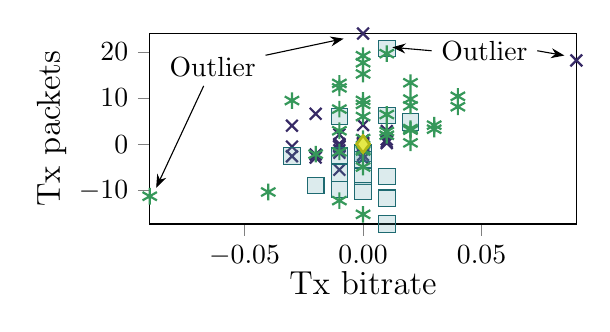
\begin{tikzpicture}

\begin{axis}[width=7cm,
height=4cm,
scaled x ticks = false,
tick align=outside,
tick pos=left,
xlabel={Tx bitrate},
xmin=-0.09, xmax=0.09,
ylabel={Tx packets},
ymin=-17.32, ymax=24,
x label style={at={(axis description cs:0.5,-0.2)},anchor=north},
xlabel style={font=\large,text depth=0pt},
ylabel style={font=\large,text depth=0pt},
%xticklabel style={font=\large},
%yticklabel style={font=\large},
%legend cell align={left},
%legend columns=-1,
%legend style={
%	%	font=\large,
%	at={(1.0,1.02)},
%	anchor=south east,
%},
colormap/viridis,
/pgf/number format/1000 sep={\,},
x tick label style={/pgf/number format/fixed,
	/pgf/number format/fixed zerofill,/pgf/number format/precision=2}
]
\addplot [mark-color=150, mark=x, only marks,thick, mark size=3pt]
table{%
	x  y
	0 0.19
	0 -0.19
	-0.03 -0.54
	-0.01 2.09
	-0.02 -2.91
	0 -0.46
	0.09 18.17
	0 24
	0.01 2.84
	-0.02 6.59
	0 4.14
	0 -2.34
	0 -3.12
	-0.01 -5.55
	-0.03 4
	-0.01 -1.87
	0 0.82
	0 -0.82
	-0.01 -0.48
	0.01 0.48
	-0.01 -0.22
	0.01 0.22
	-0.01 0.05
	-0.01 -0.53
	-0.02 -2.25
	0.01 1.04
	-0.01 -1.3
	0 0.26
	-0.03 -2.62
};
%\addlegendentry{same-prbs}
\addplot [mark-color-opacity=450,mark=square*,only marks, mark size=3pt]
table{%
	x  y
	-0.01 -6.24
	0.01 6.24
	0.02 4.85
	0 -1.98
	0 -6.87
	0.01 -11.75
	-0.01 -9.84
	0.01 -17.32
	-0.01 6.03
	-0.02 -9
	0.01 20.78
	0.01 -7.05
	0 -10.13
	-0.01 -2.5
	-0.03 -2.62
	0 -3.42
};
%\addlegendentry{same-pol}
\addplot[ mark-color=700, mark=asterisk, only marks,thick, mark size=3pt]
table{%
	x  y
	0.02 9.78
	-0.01 12.21
	0 8.63
	0.03 4.12
	0 9.49
	0 -4.96
	0.01 19.63
	0.04 10.38
	0 15.23
	0.01 6.43
	0.03 3.25
	-0.01 13.18
	0 17.66
	0 5.99
	0.02 13.32
	-0.09 -11.3
	-0.01 -12.25
	-0.03 9.46
	0.02 8.32
	0.02 0.28
	-0.01 7.61
	0 19.19
	0.01 2.74
	-0.01 2.91
	-0.04 -10.38
	0 -15.23
	0.01 1.93
	0.02 3.03
	-0.01 -1.68
	0.04 8.12
	0 1.21
	0 -1.21
	0.02 3.38
	-0.02 -2.17
	0 -1.5
};
%\addlegendentry{distinct}
\addplot [mark-color=950, mark=diamond*, only marks,thick, mark size=3pt]
table{%
	x  y
	0 0
	0 0
	0 0
	0 0
	0 0
	0 0
	0 0
	0 0
	0 0
};
%\addlegendentry{self}

%% annotations

\end{axis}
\node at (0.8,2) (out-1)  {Outlier};
\draw[-Stealth] (out-1)--++(245:1.7cm);
\draw[-Stealth] (out-1)--++(12:1.7cm);

\node at (4.25,2.2) (out-2)  {Outlier};
\draw[-Stealth] (out-2.west)--++(175:.5cm);
\draw[-Stealth] (out-2.east)--++(350:.35cm);
\end{tikzpicture}
\end{document}